\section{Model Context Protocol}
\label{sec:mcp}

The Model Context Protocol (MCP) is an open protocol developed by Anthropic that standardizes the connection between Large Language Models and external data sources, tools, and services \cite{anthropic2024mcp, mcpspec2024}. MCP provides a unified interface for exposing functionality to AI agents, enabling modular and reusable integrations that can be shared across different applications. This section examines the protocol architecture, communication patterns, and implementation considerations.

\subsection{Protocol Overview}

MCP addresses a fundamental challenge in building AI agents: the need to connect language models to diverse external systems while maintaining security, modularity, and ease of development. Prior to MCP, each integration required custom implementation, leading to fragmented ecosystems and duplicated effort.

The protocol defines a client-server architecture where:
\begin{itemize}
    \item \textbf{MCP Hosts} are applications that embed AI capabilities and initiate connections to servers
    \item \textbf{MCP Clients} are protocol implementations within hosts that maintain server connections
    \item \textbf{MCP Servers} are lightweight programs that expose specific capabilities through the protocol
\end{itemize}

% Placeholder: MCP architecture diagram
\begin{figure}[H]
    \centering
    % \fbox{\parbox{0.8\textwidth}{\centering \textit{[Placeholder: Diagram showing MCP Host, Client, and Server relationships with communication flows]}}}
    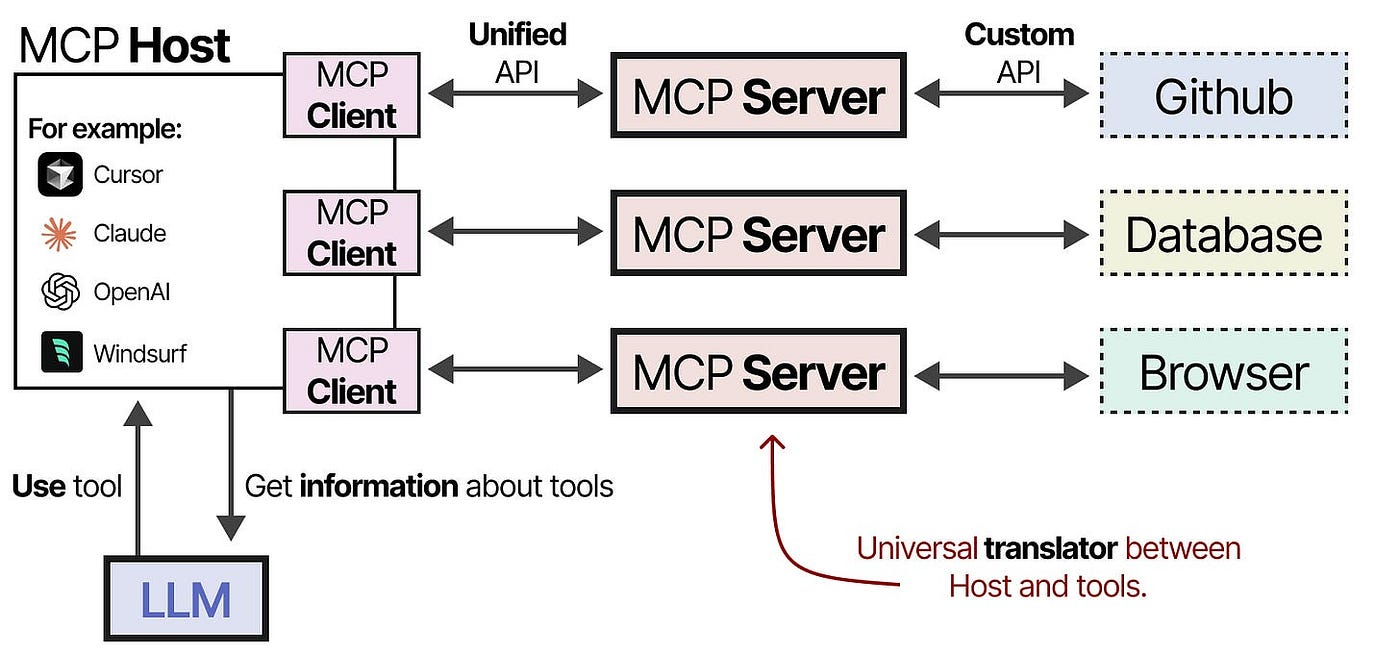
\includegraphics[width=0.7\textwidth]{images/mcp_architecture.png}
    \caption{Model Context Protocol Architecture}
    \label{fig:mcp-architecture}
\end{figure}

MCP servers can expose three types of capabilities:

\textbf{Resources} provide data that can be loaded into the model's context. Resources are identified by URIs and can represent files, database records, API responses, or any other data the model might need to reference. Resources support subscriptions for change notifications.

\textbf{Tools} represent executable functions that the model can invoke to perform actions. Each tool has a defined name, description, and parameter schema that the model uses to determine when and how to call the tool. Tools are the primary mechanism for enabling agent actions.

\textbf{Prompts} are reusable templates that encapsulate specific interaction patterns. Servers can expose prompts that provide structured ways to interact with their capabilities, helping users leverage complex functionality effectively.

\subsection{Transport Mechanisms}

MCP supports multiple transport mechanisms for client-server communication, allowing flexibility in deployment scenarios:

\textbf{Standard I/O (stdio)} is the primary transport for local servers. The host spawns the server as a subprocess and communicates through standard input/output streams. This approach provides process isolation and is well-suited for command-line tools and local integrations.

\textbf{HTTP with Server-Sent Events (SSE)} enables remote server deployment. The client connects to the server over HTTP, with the server streaming responses using SSE. This transport supports network-based architectures and allows servers to be deployed as services.

The protocol uses JSON-RPC 2.0 as the message format, providing a standardized structure for requests, responses, and notifications. Messages include method names, parameters, and result data according to the JSON-RPC specification.

\subsection{Tool Definition and Invocation}

Tools are defined using JSON Schema to specify their parameter structure. A tool definition includes:
\begin{itemize}
    \item A unique name identifying the tool
    \item A description explaining the tool's purpose and usage
    \item An input schema defining required and optional parameters
\end{itemize}

When a client connects, it queries available tools using the \texttt{tools/list} method. The server responds with the complete set of tool definitions, which the client provides to the language model as part of the function calling context.

Tool invocation follows this sequence:
\begin{enumerate}
    \item The language model determines that a tool call is needed and generates the call with arguments
    \item The client application receives the tool call request
    \item The client invokes the tool on the MCP server using the \texttt{tools/call} method
    \item The server executes the tool logic and returns results
    \item The client passes results back to the language model for incorporation
\end{enumerate}

\subsection{Implementation Patterns}

Implementing an MCP server involves creating handlers for protocol methods and defining the capabilities to expose. Common implementation patterns include:

\textbf{Wrapper servers} expose existing command-line tools or APIs through MCP. The server translates MCP tool calls into appropriate system commands or API requests, returning formatted results. This pattern enables rapid integration of existing functionality.

\textbf{Aggregator servers} combine multiple underlying services into a coherent capability set. The server manages connections to backend systems and presents a unified interface to the AI agent.

\textbf{Stateful servers} maintain context across tool invocations. While individual tool calls are stateless in the protocol, servers can maintain internal state for complex multi-step workflows.

Error handling in MCP follows standard patterns: servers return structured error responses with error codes and messages. Clients should handle both transport-level failures and application-level errors gracefully.

\subsection{Security Considerations}

MCP implementations must address several security concerns:

\textbf{Input validation}: All tool parameters must be validated before execution to prevent injection attacks or malformed inputs.

\textbf{Capability restriction}: Servers should expose only the minimum necessary functionality and implement appropriate access controls.

\textbf{Output sanitization}: Results returned to the language model should be sanitized to prevent information leakage or injection of malicious content.

\textbf{Transport security}: Remote deployments should use TLS encryption to protect data in transit.

The protocol itself does not mandate specific security mechanisms, leaving implementation decisions to developers based on their deployment context and requirements.
